\documentclass[french]{article}
 
\usepackage[utf8]{inputenc}
\usepackage[T1]{fontenc}
\usepackage{babel}
\usepackage{graphicx}
\usepackage{amsmath} 
\begin{document}
 
\section{Couche limite}

\begin{figure}[ht]
	\centering
	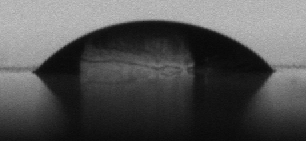
\includegraphics[scale = 0.6]{./image/crop_vitesse=28_volume=003.png}
	\caption{Goutte d'eau de volume $0.03$ml}
\end{figure}
Notre goutte d'eau (de volume de l'ordre millilitre) est sur une paroi horizontale en présence d'un écoulement d'air.


Pour déterminer les vitesses de l'écoulement d'air au voisinage de notre goutte d'eau, nous devons nous intéresser à la couche limite parce que d'après la théorie sur la couche limite, l'écoulement d'un fluide en présence d'une paroi peut être séparé en deux régions dont l'une proche de la paroi où les effets visqueux ne peuvent être négligés par rapport aux effets inertiels et l'autre région à l'extérieur de la précédente (avec une frontière commune) où les effets visqueux peuvent être négligés.

La couche limite est cette région proche de la paroi où les effets visqueux ne peuvent être négligés.

C'est Prandtl qui fut le premier à définir la couche limite. 

\subsection{Équations de la couche limite }

Les équations de la couche limite sont définies pour un écoulement bidimensionnel et nous nous les donnerons uniquement pour le cas d'un écoulement laminaire puisque nos écoulements étaient laminaires dans nos expériences.

Soit $u$ la vitesse de l'écoulement parallèle à la paroi suivant l'axe $x$ et $v$ la vitesse normale à la paroi suivant l'axe $y$.

Soit $U$ et $V$ les vitesses caractéristiques dans la couche limite respectivement de $u$ et $v$ ($\left| u \right| \sim U$ et $\left| v \right| \sim U$).

Soit $L$ et $\delta$ la taille caractéristique de la couche limite suivant respectivement l'axe $x$ et l'axe $y$ ($\left| x \right| \sim L$ et $\left| y \right| \sim \delta$).

En plus de l'hypothèse d'écoulement bidimensionnel, les hypothèses faites sont : la pesanteur est négligée, l'écoulement est stationnaire, incompressible, $\frac{\delta}{L} << 1$ et les effets visqueux et inertiels sont du même ordre de grandeur dans la couche limite.



l'équation de la continuité s'écrit alors:

\begin{equation}
\label{Eq:1}
\frac{\partial u}{\partial x} + \frac{\partial v}{\partial y} = 0
\end{equation}


L'équation de Navier-Stokes s'écrit:

\begin{align}%[Navier, Stokes]
	u\frac{\partial u}{\partial x} + 
	v\frac{\partial u}{\partial y} 
	&= - \frac{1}{\rho}
	\frac{\partial p}{\partial  x} +
	\nu\left (
	\frac{\partial^{2} u}{\partial  x^{2}} + 
	\frac{\partial^{2} u}{\partial  y^{2}}
	\right ) \\
	u\frac{\partial v}{\partial x} + 
	v\frac{\partial v}{\partial y} 
	&= - \frac{1}{\rho}
	\frac{\partial p}{\partial  y} +
	\nu\left (
	\frac{\partial^{2} v}{\partial  x^{2}} + 
	\frac{\partial^{2} v}{\partial  y^{2}}
	\right ) 
\end{align}

On pose:

\begin{align*}
	u &= Uu_{*}\\
	v &= Vv_{*}\\
	x &= Lx_{*}\\
	y &= \delta y_{*}\\
	p &= \lambda p_{*}
\end{align*}
Avec pour tout entier  $n >= 0$:
\begin{align*}
	\left| u_{*} \right |,
	\left| v_{*} \right |,
	\left| p_{*} \right | 
	&\sim 1\\
	\left |\frac{\partial^{n} u_{*}}{\partial x_{*}^{n}} \right |,
	\left |\frac{\partial^{n} v_{*}}{\partial x_{*}^{n}} \right |,
	\left |\frac{\partial^{n} p_{*}}{\partial x_{*}^{n}} \right |
	&\sim 1\\
	\left |\frac{\partial^{n} u_{*}}{\partial y_{*}^{n}} \right |,
	\left |\frac{\partial^{n} v_{*}}{\partial y_{*}^{n}} \right |,
	\left |\frac{\partial^{n} p_{*}}{\partial y_{*}^{n}} \right |
	&\sim 1
\end{align*}
Les équations de Navier-Stokes se réécrivent :
\begin{align*}
	\frac{U^{2}}{L}
	u_{*}
	\frac{\partial u_{*}}{\partial x_{*}} + 
	\frac{UV}{\delta}
	v_{*}
	\frac{\partial u_{*}}{\partial y_{*}} 
	&= - \frac{\lambda}{\rho L}
	\frac{\partial p_{*}}{\partial  x_{*}} +
	\nu 
	\left(
	\frac{U}{L^{2}}
	\frac{\partial^{2} u_{*}}{\partial  x_{*}^{2}} + 
	\frac{U}{\delta ^ {2}}
	\frac{\partial^{2} u_{*}}{\partial  y_{*}^{2}}
	\right) \\
	\frac{UV}{L}
	u_{*}
	\frac{\partial v_{*}}{\partial x_{*}} + 
	\frac{V^{2}}{\delta}
	v_{*}
	\frac{\partial v_{*}}{\partial y_{*}} 
	&= 
	- \frac{\lambda}{\rho\delta}
	\frac{\partial p_{*}}{\partial  y_{*}} +
	\nu
	\left(
	\frac{V}{L^{2}}
	\frac{\partial^{2} v_{*}}{\partial  x_{*}^{2}} + 
	\frac{V}{\delta^{2}}
	\frac{\partial^{2} v_{*}}{\partial  y_{*}^{2}}
	\right) 
\end{align*}
De l'hypothèse $\frac{\delta}{L} << 1 $, on a:
\begin{align*}
	\frac{\delta}{L} &<< 1\\
	\frac{U}{L^{2}}\frac{\partial^{2} u_{*}}{\partial  x_{*}^{2}} 
	&<<
	\frac{U}{\delta ^ {2}}
	\frac{\partial^{2} u_{*}}{\partial  y_{*}^{2}} \\
	\frac{V}{L^{2}}
	\frac{\partial^{2} v_{*}}{\partial  x_{*}^{2}} 
	&<<
	\frac{V}{\delta^{2}}
	\frac{\partial^{2} v_{*}}{\partial  y_{*}^{2}}
\end{align*}

L'équation de continuité nous dit:

\begin{equation*}
	\frac{V}{\delta} \sim \frac{U}{L}
\end{equation*}

En conservant les termes dominants et de $\frac{V}{\delta} \sim \frac{U}{L}$, l'équation de Navier-Stokes s'approxime par:
\begin{align*}
	\frac{U^{2}}{L}
	\left(
	u_{*}\frac{\partial u_{*}}{\partial x_{*}} + 
	v_{*}\frac{\partial u_{*}}{\partial y_{*}} 
	\right)
	&= - \frac{\lambda}{\rho L}
	\frac{\partial p_{*}}{\partial  x_{*}} +
	\nu  \frac{U}{\delta^{2}}
	\frac{\partial^{2} u_{*}}{\partial  y_{*}^{2}} \\
	\frac{V^{2}}{\delta}
	\left(
	u_{*}\frac{\partial v_{*}}{\partial x_{*}} + 
	v_{*}\frac{\partial v_{*}}{\partial y_{*}} 
	\right)
	&= - \frac{\lambda}{\rho\delta}
	\frac{\partial p_{*}}{\partial  y_{*}} +
	\nu\frac{V}{\delta^{2}}
	\frac{\partial^{2} v_{*}}{\partial  y_{*}^{2}} 
\end{align*}
De l'hypothèse du même ordre grandeur des termes visqueux et inertiels, on a avec l'équation de Navier-Stokes selon $x$:

\begin{align*}
	\frac{U^{2}}{L} &\sim 
	\nu\frac{U}{\delta^{2}} \\
	\frac{\delta^{2}}{L} &\sim 
	\frac{\nu}{U}\\
	\frac{\delta^{2}}{L^{2}} &\sim 
	\frac{\nu}{UL} = \frac{1}{Re_{L}} << 1
\end{align*}

On constate qu'on doit avoir un nombre de Reynolds $\frac{UL}{\nu} = Re_{L}$ suffisamment grand pour vérifier les hypothèses de la couche limite ($1 << Re_{L}$).

De $ \frac{\delta^{2}}{L^{2}} \sim \frac{\nu}{UL} $  
et $ V \sim \frac{U\delta}{L}$ on a :
\begin{equation*}
	\nu \sim \frac{U\delta}{L}\delta \sim V\delta
\end{equation*}

On constate que de $\nu \sim V\delta$, les termes visqueux et inertiels suivant $y$ ont aussi le même ordre de grandeur, en effet : 

\begin{equation*}
	\frac{V^{2}}{\delta} =
	\frac{V^{2}\delta}{\delta ^ 2} =
	V\delta \frac{V}{\delta^{2}} \sim \nu \frac{V}{\delta^{2}}
\end{equation*}

Ce qui donne l'ordre de grandeur de $\frac{1}{\rho}\frac{\partial p}{\partial y} \sim \frac{V^{2}}{\delta}$ en effet:


\begin{equation*}
	\frac{1}{\rho}
	\frac{\partial p}{\partial y} 
	= \frac{\lambda}{\rho\delta}
	\frac{\partial p_{*}}{\partial  y_{*}}
	= - \frac{V^{2}}{\delta}
	\left(
	u_{*}\frac{\partial v_{*}}{\partial x_{*}} + 
	v_{*}\frac{\partial v_{*}}{\partial y_{*}} 
	-\frac{\partial^{2} v_{*}}{\partial  y_{*}^{2}} 
	\right)
\end{equation*}

Du fait que $\frac{U^{2}}{L}$ soit l'ordre de grandeur des termes de l'équation de Navier-Stokes suivant $x$ et que $\frac{V^{2}}{\delta} << \frac{U^2}{L}$ on a abouti à l'approximation:
\begin{equation*}
	\frac{1}{\rho}\frac{\partial p}{\partial y} \approx 0
\end{equation*}

Les équations de la couche limites sont donc :

\begin{align}	
	\frac{\partial u}{\partial x} 
	+
	\frac{\partial v}{\partial y} 
	&= 0 \\
	u\frac{\partial u}{\partial x} + 
	v\frac{\partial u}{\partial y} 
	&= - \frac{1}{\rho}
	\frac{\partial p}{\partial  x} +
	\nu
	\frac{\partial^{2} u}{\partial  y^{2}} \\
	\frac{\partial p}{\partial y} 
	&= 0
\end{align}
\subsection{Équations de Blasius}
L'équation de Blasius est l'équation de la couche limite pour un écoulement laminaire sur une plaque plane dont la vitesse $U$ loin de la couche limite est constante et parallèle à l'axe $x$.

Soit $\varphi$ la fonction de courant tel que :

\begin{align*}
	u(x,y) &= 
	\frac{\partial \varphi}{\partial y} \\
	v(x,y) &= - 
	\frac{\partial \varphi}{\partial x}
\end{align*}

On pose :

\begin{align*}
	\eta &= y \sqrt{\frac{U}{2\nu x }} \\
	\varphi &= \sqrt{2\nu U x} f(\eta)
\end{align*}
On a:
\begin{align*}
	\frac{\partial \eta}{\partial x} &= 
		-y\sqrt{\frac{U}{2\nu x}}\frac{1}{2x} &&= 
		-\frac{\eta}{2x}\\
		\frac{\partial \eta}{\partial y} &=
		\sqrt{\frac{U}{2\nu x }} &&= \frac{\eta}{y}\\
		\frac{\partial^{2} \eta}{\partial y^{2}} &= 
		\frac{\eta}{y^{2}} - \frac{\eta}{y^{2}} &&= 0
\end{align*}
Puis on calcule $u$ et $v$ en fonction de $f$ et $\eta$.
\begin{align*}
	u(x,y) &= 
	\frac{\partial \varphi}{\partial y} 
	=
	\sqrt{\frac{U}{2\nu x }} \sqrt{2\nu U x}\frac{d f}{\partial \eta}
	= U \frac{d f}{\partial \eta}\\
	\\
	v(x,y) &= 
	- \frac{\partial \varphi}{\partial x} \\
	&=
	-\frac{\partial \sqrt{2\nu U x}} {\partial x}
	f(\eta) -
	\sqrt{2\nu Ux }
	\frac{\partial f(\eta)}{\partial x}\\
	&= 
	-\sqrt{\frac{\nu U}{2x}}
	f(\eta) -
	\sqrt{2\nu Ux }
	\frac{\partial f}{\partial \eta}
	\frac{\partial \eta}{\partial x}\\
	&=
	-\sqrt{\frac{\nu U}{2x}}
	f(\eta) +
	\sqrt{2\nu Ux}\frac{\eta}{2x}\frac{d f}{d \eta}
	\\
	&=
	-\sqrt{\frac{\nu U}{2x}}
	f(\eta) +
	\sqrt{\frac{\nu U}{2x}}\eta\frac{d f}{d \eta}
	\\
	&=
	\sqrt{\frac{\nu U}{2x}}
	\left(
	-f(\eta) + \eta\frac{d f}{d \eta}
	\right)
\end{align*}

On obtient:

\begin{align}
	u(x,y) &= 
	 U \frac{d f}{d \eta}\\
	v(x,y) &= 
	\sqrt{\frac{\nu U}{2x}}
	\left(
	-f(\eta) + \eta\frac{d f}{d \eta}
	\right) = 
	\frac{\nu\eta}{y}
	\left(
	-f(\eta) + \eta\frac{d f}{d \eta}
	\right)
\end{align}

De $\frac{\partial p}{\partial y} = 0$ qui nous dit que la pression ne dépend que de $x$ ($p = p(x)$) et de l'équation de Bernouilli loin de la couche limite où la vitesse est constante et vaut $U$ on a:


\begin{equation*}
	\frac{p(x)}{\rho} + \frac{U^2}{2} = constante
\end{equation*}
Comme $U = constante$, on a $p = constante$ et en particulier:
\begin{equation}
	\frac{\partial p}{\partial x}  = 0
\end{equation}

Et en remplaçant $u$ et $v$ dans l'équation de Navier-Stokes de la couche limite suivant $x$, on obtient:


\begin{align*}	
	u\frac{\partial u}{\partial \eta}
	\frac{\partial \eta}{\partial x} + 
	v\frac{\partial u}{\partial \eta} 
	\frac{\partial \eta}{\partial y}
	&= \nu\left(
	\frac{\partial^{2} u}{\partial  \eta^{2}}
	\left(
	\frac{\partial \eta}{\partial  y}
	\right)^{2} +
	\frac{\partial u}{\partial  \eta}
	\frac{\partial^{2} \eta}{\partial  y^{2}}
	\right)\\
	u\frac{\partial u}{\partial \eta}
	\frac{\partial \eta}{\partial x} + 
	v\frac{\partial u}{\partial \eta} 
	\frac{\partial \eta}{\partial y}
	&= \nu
	\frac{\partial^{2} u}{\partial  \eta^{2}}
	\left(
	\frac{\partial \eta}{\partial  y}
	\right)^{2} \\
	-U\frac{U}{2x} 
	\eta
	\frac{d f}{d \eta}
	\frac{d^{2} f}{d \eta^{2}}
	+ 
	\nu
	\frac{U\eta^{2}}{y^{2}}
	\left(
	-f(\eta) + \eta\frac{d f}{d \eta}
	\right)
	\frac{d^{2} f}{d \eta^{2}} 
	&= \nu
	\frac{U\eta^{2}}{y^{2}}
	\frac{d^{3} f}{d\eta^{3}}
\end{align*}
De $\eta = y \sqrt{\frac{U}{2\nu x }}$, on a $
	\frac{U}{2x} = \nu 
	\frac{\eta^{2}}{y^{2}}
$ et : 
\begin{align*}	
	-\nu
	\frac{U\eta^{2}}{y^{2}} 
	\eta
	\frac{d f}{d \eta}
	\frac{d^{2} f}{d \eta^{2}}
	+ 
	\nu
	\frac{U\eta^{2}}{y^{2}}
	\left(
	-f(\eta) + \eta\frac{d f}{d \eta}
	\right)
	\frac{d^{2} f}{d \eta^{2}} 
	&= \nu
	\frac{U\eta^{2}}{y^{2}}
	\frac{d^{3} f}{d\eta^{3}}
\end{align*}

On trouve ainsi l'équation de la couche limite de Blasius:
\begin{equation}	
	\frac{d^{3}f}{d\eta^{3}} + f\frac{d^{2} f}{d\eta^{2}}
\end{equation}
Avec les conditions aux limites:
\begin{align}
	u(x,0) &= 0 &\Rightarrow &&
	\left.
	\frac{d f}{d \eta}     \right|_{\eta = 0} &= 0
	\\
	v(x,0) &= 0 &\Rightarrow &&
	f(0) &= 0
	\\
	u(x,\infty) &= U &\Rightarrow &&
	\left.
	\frac{d f}{d \eta} \right|_{\eta = \infty} &= 1
\end{align}
\newpage
\begin{figure}[ht]
	\centering
	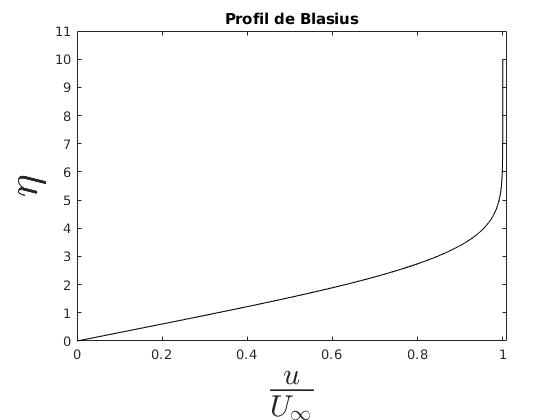
\includegraphics[scale = 0.6]{./image/Blasius.png}
	\caption{Profil de Blasius}
\end{figure}
Les grandeurs que nous avons comparées expérimentalement provenant du résultat des équations de Blasius sont l'épaisseur de déplacement $\delta_{1}$, l'épaisseur de quantité de mouvement $\delta_{2}$ et le coefficient de frottement $C_{f}$
\subsection{Épaisseur de déplacement}
L'épaisseur de déplacement $\delta_{1}$ à $x$ fixé est définie par:
\begin{equation}
	\delta_{1} = 
	\int_{0}^{^\infty}
	\left(
	1 - 
	\frac{u}{U}
	\right)
	dy
\end{equation}
\begin{align*}
	\delta_{1} &= 
	\int_{0}^{^\infty}
	\left(
	1 - 
	\frac{u}{U}
	\right)
	dy\\
	&= \int_{0}^{\infty}
	\left(
	1 - \frac{df}{d\eta}
	\right)
	dy 
	= \int_{0}^{\infty}
	\left(
	1 - \frac{df}{d\eta}
	\right)
	\frac{\partial y}{\partial \eta}d\eta\\
	&= \sqrt{\frac{2\nu x}{U}}
	\int_{0}^{\infty}
	\left(
	1 - \frac{df}{d\eta}
	\right)
	d\eta\\
	&= x\sqrt{\frac{2}{Re_{x}}}
	\left(
	\lim_{\eta\to\infty}
	\left(
	\eta - f(\eta)
	\right)
	\right)
\end{align*}
$ \lim_{\eta\to\infty}\left(\eta - f(\eta)\right)$ est évalué numériquement et on trouve:
\begin{equation}
	\delta_{1}(x)	\approx \frac{1.72x}{\sqrt{Re_{x}}}
\end{equation}
\subsection{Épaisseur de quantité de mouvement}
L'épaisseur de quantité de mouvement $\delta_{2}$ à $x$ fixé est définie par:
\begin{equation}
	\delta_{2} = 
	\int_{0}^{^\infty}
	\frac{u}{U}
	\left(
	1 - 
	\frac{u}{U}
	\right)
	dy
\end{equation}
\begin{align*}
	\delta_{2} &= 
	\int_{0}^{^\infty}
	\frac{u}{U}
	\left(
	1 - 
	\frac{u}{U}
	\right)
	dy\\
	&= \int_{0}^{\infty}
	\frac{df}{d\eta}
	\left(
	1 - \frac{df}{d\eta}
	\right)
	\frac{\partial y}{\partial \eta}d\eta\\
	&= \sqrt{\frac{2\nu x}{U}}
	\int_{0}^{\infty}
	\frac{df}{d\eta}
	\left(
	1 - \frac{df}{d\eta}
	\right)d\eta\\
	&= x\sqrt{\frac{2}{Re_{x}}}
	\int_{0}^{\infty}
	\frac{df}{d\eta}
	\left(
	1 - \frac{df}{d\eta}
	\right)d\eta
\end{align*}
$ \int_{0}^{\infty}
\frac{df}{d\eta}
\left(1 - \frac{df}{d\eta}\right)d\eta$ est évalué numériquement et on trouve:
\begin{equation}
	\delta_{2}(x)	\approx \frac{0.664x}{\sqrt{Re_{x}}}
\end{equation}
\subsection{Coefficient de frottement à la paroi}
Le coefficient de frottement à la paroi $C_{f}$ à $x$ fixé est défini par:
\begin{equation}
	C_{f} =
	\frac{2\tau_{y=0}}{\rho U^{2}} =
	\frac{2\nu}{U^{2}}
	\left.
	\frac{\partial u}{\partial y}
	\right|_{y = 0}
\end{equation}
\begin{align*}
	C_{f} &= 
	\frac{2\nu}{U^{2}}
	\left.
	\frac{\partial u}{\partial y}
	\right|_{y = 0}
	&&= \frac{2\nu}{U^{2}}
	 U\sqrt{\frac{U}{2\nu x}}
	\left.
	\frac{d^{2}f}{d\eta^{2}}
	\right|_{\eta = 0}\\
	&= \frac{2\nu}{U}
	 \sqrt{\frac{U}{2\nu x}}
	\left.
	\frac{d^{2}f}{d\eta^{2}}
	\right|_{\eta = 0}
	&&= 
	 \sqrt{\frac{2}{Re_{x}}}
	\left.
	\frac{d^{2}f}{d\eta^{2}}
	\right|_{\eta = 0}
\end{align*}
$ \left. \frac{d^{2}f}{d\eta^{2}} \right|_{\eta = 0} $ est évalué numériquement et on trouve:
\begin{equation}
	C_{f}(x) \approx \frac{0.664}{\sqrt{Re_{x}}}
\end{equation}
\subsection{Comparaisons avec nos expériences}
Nous avons effectué nos mesures à l'aide de l'anémomètre à fil chaud et nous trouvons avec :
\begin{align*}
	x &= 0.55m\\
	Re_{x} &= \frac{Ux}{\nu}\\
	\nu &= 1.5e-5 m^{2}.s^{-1}~~\text{à}~~T = 25^{o}C; 
\end{align*}
\begin{table}[ht]
	\centering
	\begin{tabular}{cc}
		\hline\\
		$U(m/s)$ & Reynolds\\
		\hline
   15 & 5.5000000e+05\\
   20 & 7.3333333e+05\\
   24 & 8.8000000e+05\\
   28 & 1.0266667e+06
	\end{tabular}
	\caption{Nombre de Reynolds $Re_{x}$}
\end{table}
\begin{table}[ht]
	\centering
	\begin{tabular}{cccc}
		\hline\\
		$U(m/s)$ & $\delta_{1Blasius}(m)$ &
		$ \delta_{1Experience}(m)$ & 
		 erreur relative\\
		\hline
		15   & 1.2708977e-03   & 1.2366791e-03   & 2.69\%\\
		20   & 1.1077156e-03   & 1.1009662e-03   & 0.61\%\\
		24   & 1.0253841e-03   & 9.9332014e-04   & 3.13\%\\
		28   & 9.6219321e-04   & 9.4728404e-04   & 1.55\%
	\end{tabular}
	\caption{Comparaison épaisseur de déplacement $\delta_{1}$}
\end{table}
\begin{table}[ht]
	\centering
	\begin{tabular}{cccc}
		\hline\\
		$U(m/s)$ & $\delta_{2Blasius}(m)$ &
		$ \delta_{2Experience}(m)$ & 
		 erreur relative\\
		\hline
   15 & 4.9062563e-04   & 4.7278049e-04   & 3.64\%\\
   20 & 4.2762976e-04   & 4.0788245e-04   & 4.62\%\\
   24 & 3.9584594e-04   & 3.7179338e-04   & 6.08\%\\
   28 & 3.7145133e-04   & 3.4572931e-04   & 6.92\%
	\end{tabular}
	\caption{Comparaison épaisseur de quantité de mouvement $\delta_{2}$}
\end{table}
\begin{table}[ht]
	\centering
	\begin{tabular}{cccc}
		\hline\\
		$U(m/s)$ & $C_{fBlasius}$ &
		$ C_{fExperience}$ & 
		 erreur relative\\
		\hline
   15 & 8.9204661e-04   & 9.1781966e-04   & 2.89\%\\
   20 & 7.7750866e-04   & 7.6736042e-04   & 1.31\%\\
   24 & 7.1971988e-04   & 7.3306205e-04   & 1.85\%\\
   28 & 6.7536606e-04   & 6.6688383e-04   & 1.26\%
	\end{tabular}
	\caption{Comparaison coefficient de frottement $C_{f}$}
\end{table}
\begin{figure}[ht]
	\centering
	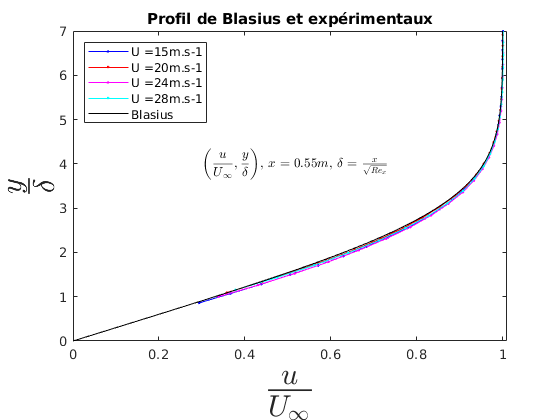
\includegraphics[scale = 0.6]{./image/Bla.png}
	\caption{Profil de Blasius et expérimentaux}
\end{figure}
%\begin{thebibliography}{}
%\bibitem{RefJ}
%% Format for Journal Reference
%Author, Article title, Journal, Volume, page numbers (year)
%% Format for books
%\bibitem{RefB}
%Author, Book title, page numbers. Publisher, place (year)
%\end{thebibliography}
\end{document}
